
\chapter{Background} \label{bgrnd}

Our system builds on a lot of existing technology.
To lay the foundation of the thesis we first discuss some computer graphics fundamentals (Section \ref{els}).
We then describe level-of-detail algorithms, a fundamental basis for most of the work in the system (Section \ref{lod}).
Next, we discuss some methods for generating and rendering terrain (Sections \ref{terrain_gen} and \ref{terrain_render} respectively), including a look at voxel terrain in particular (Section \ref{voxels}).
Finally, we give an overview of a rendering effect used to improve the appearance of our renders (Section \ref{ssao}).


\section{The Many Els} \label{els}

Many computer graphics techniques involve breaking down complex objects into a large number of individual elements.
As such, we need terminology to refer to these different types of elements.

Perhaps the most commonly known individual element is a pixel.
The term pixel refers to a ``\textbf{Pi}cture \textbf{El}ement''.
In this case, a picture has been broken down into its individual elements, pixels.
In this paper, we will discuss pixels and other such elements including:

\begin{itemize}
	\item Texels ``\textbf{Tex}ture \textbf{El}ements''
	\item Surfels ``\textbf{Surf}ace \textbf{El}ements''
	\item Voxels ``\textbf{Vo}lume \textbf{El}ements''
\end{itemize}


\section{Level of Detail} \label{lod}

There are several limitations when it comes to rendering large scenes.
In general, the large amount of geometry required to represent these scenes is at odds with the limited resources of the computer.
The GPU is only able to render and shade a certain amount of geometry due to processor speed and number of available processors.
Scene geometry must be loaded into main memory, then transferred to graphics memory, both of which have throughput maximums and storage maximums.
The hardware interface also has some CPU overhead with regard to submitting draw commands, so we are limited in the number of draw calls we can make.

As such, in order to render large scenes with a large number of scene elements, we need to account for level of detail.
`Detail' in this context refers generally to the amount of geometry used to represent a scene element.
Consider, for example, a tree.{}
A high-detail representation of a tree would consist of geometry to represent branches, individual leaves, and the shape of the trunk.
A low-detail representation of a tree might simply consist of a trunk-colored box and a leaf-colored cone.
See Figure~\ref{fig:trees} for an example of these representations.

\begin{figure}
	\centering
		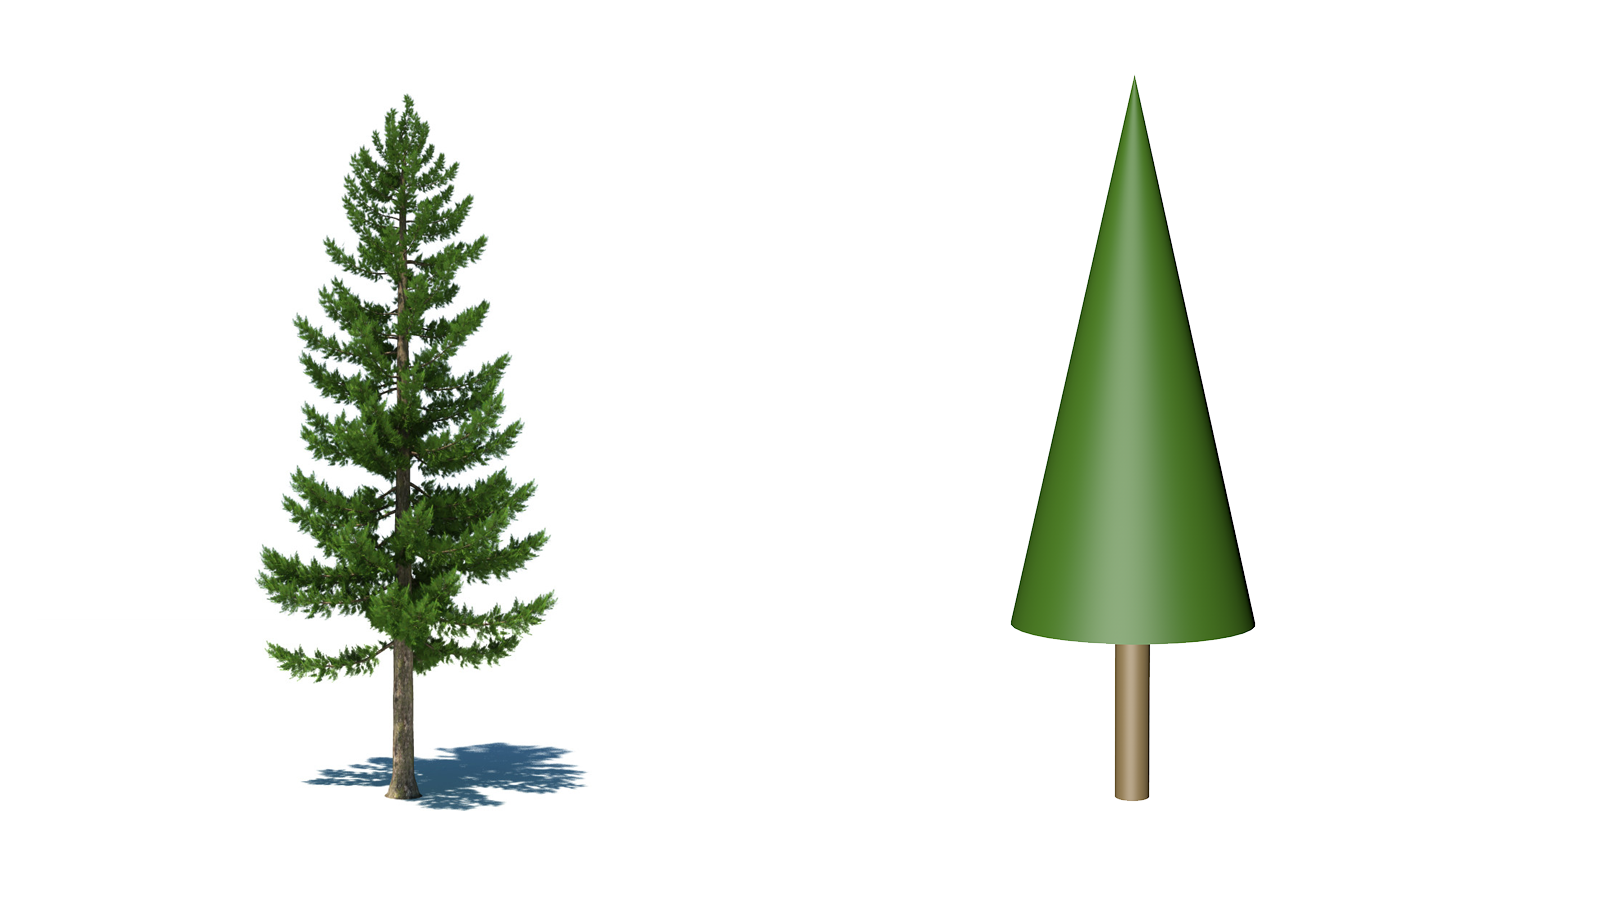
\includegraphics[width=1.0\textwidth]{figures/TreeComparison.png}
	\caption{On the left is an example of a high-detail tree, on the right is a low-detail tree.
	While the low detail approximation may appear very crude, it is a reasonable substitution when the tree is so distant that it takes up only a few pixels of screenspace.}
	\label{fig:trees}
\end{figure}


Smaller details like branches and individual leaves are no longer visible in the low-detail representation, but are represented more abstractly by the box and cone shapes.
The advantage of the low-detail representation is that it requires fewer resources to draw.

In addition, it is also a bad idea to render distant scene elements at full-detail even if resources are available.
The farther away a scene element is from the viewpoint, the smaller it is in terms of screen-space.
Drawing primitives that are smaller in terms of screen-space can cause aliasing, a visual artifact.
As such, low-detail representations can sometimes appear better than their high-detail counterparts at large view distances.

Level-of-detail is commonly abbreviated LOD.
A rendering system that is capable of representing scene elements in both high-detail and low-detail formats is referred to as a LOD rendering system.
A LOD system must switch freely between these representations as the viewpoint changes to reduce the amount of geometry and draw calls required to render a large scene, while still representing nearby objects at full detail.

One common LOD system that is implemented in most graphics hardware is texture mipmapping \cite{opengl_mipmaps}.


\section{Terrain Rendering} \label{terrain_render}

Terrain rendering is a prime candidate for using a level-of-detail algorithm because terrain consists of a large amount of geometry and is visible both up close and at large view distances.
Over the years there have been many published techniques for terrain rendering
\cite{hardware_lod}
\cite{roambetter}
\cite{bruneton_terrain}
\cite{p-bdam}
\cite{righttri}
\cite{diamondterrain}
\cite{roam}
\cite{clod}.
However, we will focus on some more modern techniques that serve as the basis for the terrain system presented in this paper.


\subsection{Heightmaps}

A common technique for simplifying terrain representation is the use of a heightmap.
A heightmap is based on the assumption that terrain elevation is uniformly sampled, i.e. we know the height of the terrain at evenly spaced intervals.
Instead of storing a set of 3D points to represent the terrain surface, we can instead create a generic 2D regular grid and store the height separately.
This separate array of height values is referred to as a heightmap.
See Figure~\ref{fig:hm} for an example of a heightmap.

\begin{figure}
	\centering
		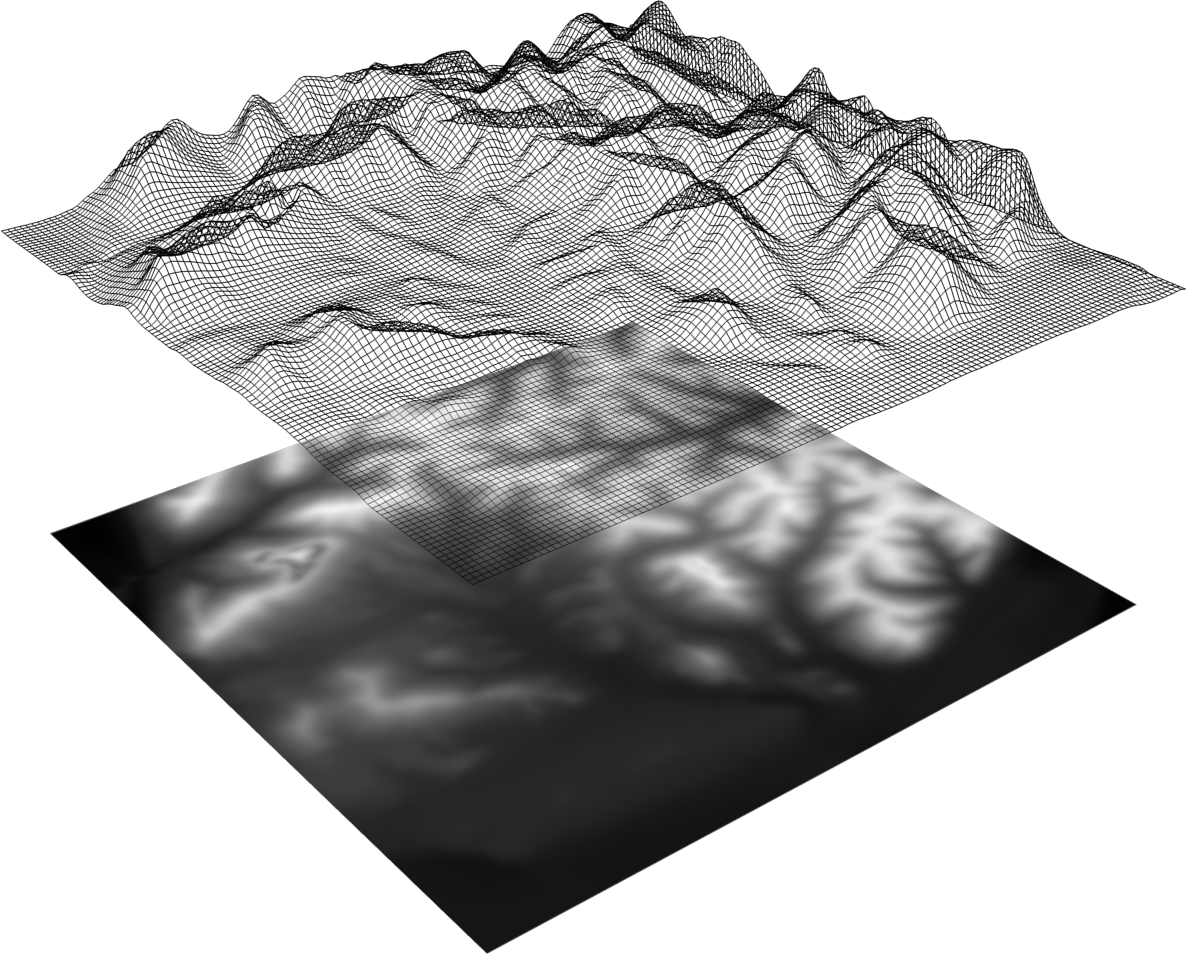
\includegraphics[width=0.6\textwidth]{figures/hm1.png}
	\caption{An example of a heightmap (below) and its respective terrain (above).}
	\label{fig:hm}
	% https://www.ssucet.org/~jhudson/15/2802/heightmap/hm1.png
\end{figure}

\subsection{Geometry Clipmaps}

Geometry clipmaps is a terrain rendering technique from 2004 that uses a series of nested regular grids to represent each detail level of the terrain \cite{geometry_clipmaps}.
A regular grid of terrain at maximum detail is centered around the viewpoint.
Another regular grid of terrain at twice the scale (and thus half resolution) is centered around that inner grid, but with a hole cut out where the inner grid is located.
Thus the second grid is clipped by the first grid (i.e. a clipmap).
Consecutive grids are added in the same manner, each twice the scale and half the resolution of the previous.
Each of these grids is referred to as a layer.
The geometry clipmaps approach also includes a system for blending the low and high detail representations at layer boundaries, and for updating the heightmaps used by each layer.
Heightmaps are updated toroidally so that small incremental updates are possible as the viewpoint moves.
See Figures \ref{fig:toroid} and \ref{fig:clipmaps_update}.

\begin{figure}
	\centering
		
\includegraphics[width=0.5\textwidth]{figures/toroid.png}
	\caption{
		An interesting property of a toroid is that moving along either direction of gridlines will eventually lead you back to your starting point.
		This concept is used to perform incremental updates to the heightmaps in geometry clipmaps.
	}
	\label{fig:toroid}
	% https://qph.ec.quoracdn.net/main-qimg-29e8370d1edfe01c997d43ae6930dd6a?convert_to_webp=true
\end{figure}

\begin{figure}
	\centering
		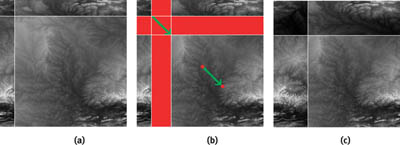
\includegraphics[width=1.0\textwidth]{figures/clipmaps_update.jpg}
	\caption{
		An example of a toroidal update for a geometry clipmaps heightmap.
		Image (b) shows how the movement of the viewpoint causes the red region to be updated.
	}
	\label{fig:clipmaps_update}
	% http://http.developer.nvidia.com/GPUGems2/elementLinks/02_geoclipmaps_08part1.jpg
\end{figure}

More recently, work has been done on improving the geometry clipmaps technique for use with modern rendering hardware, but the principles remain the same \cite{gems_clipmaps}.

The system in this paper uses a modified version of geometry clipmaps, which is discussed in Section \ref{clipterrain}.

\section{Terrain Generation} \label{terrain_gen}

Before addressing the problem of how to render terrain we must first decide where our terrain data will come from.

There are many possible sources of terrain data.
Acquired data from the real world is often available.
The USGS provides satellite data for much of the world's surface.
Some game engines also use terrain editing tools that allow artists to sculpt terrain manually.

It is also possible to implement algorithms that procedurally construct terrain.
The advantage of using procedurally generated terrain is that it requires less time and effort  than artistically creating a terrain, and it does not require much or any disk space (as opposed to using acquired data which can be very large).

Procedural terrain generation methodologies usually employ one or more of the follow techniques.

\begin{itemize}
\item Physical process simulations
\item Fractal processes
\item Noise algorithms
\end{itemize}

\subsection{Physical process simulations}

Real terrain is shaped by erosion, the gradual shaping of landscape caused by water, wind, and other forces.
Some terrain generation techniques simulate these physical processes on a starter dataset to create realistic surfaces \cite{hydrology}.

However, the nature of the physical simulation usually requires the entire world (or at least individual continents) to be generated at once.
This means that the generation of very large worlds can be very expensive in terms of both processing time and memory requirements.

Physical process simulations are often used in fields where time and memory requirements are not as stringent, e.g. offline rendering for movies.


\subsection{Fractal processes}

Another technique for generating terrain is a fractal process, some algorithm that operates on geometry to add detail and which can be re-applied at smaller and smaller scale until a highly detailed surface results.
One common form of fractal process is the Diamond-square Algorithm which sequentially subdivides and modulates a regular grid \cite{def_rend_terrain}.


\subsection{Noise Algorithms}

Noise algorithms are similar to fractal processes but do not need to operate on a regular grid of fixed size \cite{perlin}.
The most typical way that noise algorithms are used is by generating a patch or formula for noise (typically in two dimensions, though sometimes more) and employing a technique called fractional Brownian motion to create a heightmap.
The primary advantage of noise terrain generation over the previous two methods is that the generation of an individual elevation value is entirely independent of neighboring values.
This means that a noise algorithm can be more easily parallelized, and applied more effectively for use with a LOD terrain rendering system.

Noise is generally a signal that varies randomly.
Coherent noise is a special brand of noise that is more useful for generation purposes.
As a random signal, it is reasonable to expect that a large change in domain results in a random change in output for a given noise function.
Coherent noise has the property that for small changes in domain, only a small change in output will result.



\subsubsection{Coherent Noise}

There are two major types of coherent noise.

% \subsubsection{Value noise}

The most simple is value noise.
Value noise is generated by calculating random numbers at fixed intervals and interpolating between the values.

% Value noise works by using a pseudo-random number generator to generate a set of initial random values, then interpolate between those values.

% \subsubsection{Gradient noise}

Another type of coherent noise is gradient noise.
Gradient noise is generated by calculating vectors at a fixed interval, then performing a dot product to calculate intermediary values instead of interpolating.
It is a numerically similar process to value noise, but produces noise with more variance - that is, more detail in higher frequencies.

% Gradient noise is a modification of value noise where gradient vectors are calculated at grid points, and noise is generated by calculating the dot product between a gradient vector and the offset to the calculated location.
% The purpose of this technique is the improve the mathematical properties of the

\subsubsection{Fractal Noise}

Fractal noise, or \(1/f\) noise, is a technique for taking a noise function and adding detail at higher frequencies \cite{perlin}.
The general approach is:
\begin{enumerate}
\item Take a noise function as input
\item Double the frequency and halve the amplitude of the noise function, then add it to itself. This is called the second octave.
\item Double again the frequency and halve again the amplitude of the noise function, then add this too into the sum. This is the third octave.
\item Repeat Step 3 for subsequent octaves until amplitude is close enough to zero that added octaves produce no change in the output, or until desired amount of detail is reached.
\end{enumerate}

In general you do not need to exactly double the frequency or halve the amplitude each octave, but can fine tune these values e.g. by multiplying the frequency by 1.2 and the amplitude by 0.3.

\subsubsection{Ridged Noise}

An additional step can be added before summing each individual octave.
By first taking the negated absolute value of each generated noise value, a ridged version of fractional brownian motion can be created.
This technique is commonly referred to as ridged fractal generator, or sometimes a turbulence generator \cite{perlin}.

\subsubsection{Noise Distortion}

Ridged noise works on by modifying the range of each noise function, but it is also possible to modify the domain in a similar fashion.
Using two additional fractal generators, an offset vector can be produced for each sample of the height generator.
This technique helps break up the homogeneous appearance of generated terrain by shrinking and expanding different areas.


\section{Voxels} \label{voxels}

A voxel is a three-dimensional analogue to a pixel.
While an image can be represented by a 2D array of pixels, a volume can be represented by a 3D array of voxels - see Figure \ref{fig:voxels}.

\begin{figure}
	\centering
		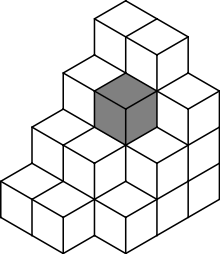
\includegraphics[width=0.3\textwidth]{figures/voxels}
	\caption{Voxels}
	\label{fig:voxels}
	% https://upload.wikimedia.org/wikipedia/commons/thumb/b/bc/Voxels.svg/220px-Voxels.svg.png
\end{figure}

Voxels are sometimes used to represent and render 3D terrain.
{\em Minecraft} is perhaps the most popular example of this technique, where the terrain and other objects are represented as voxels.

Voxels can be either converted to a polygon mesh for rendering (this is the technique used by {\em Minecraft}, or rendered more directly using ray-casting or other similar approaches.
In Section \ref{voxterrain} we discuss our approach to using voxels to represent and render terrain.


\section{Screen-space Ambient Occlusion} \label{ssao}

Without shadows, it is sometimes difficult to understand the shape and spatial orientation of rendered objects.
One way to add simple shadows to a scene is by accounting for the occlusion of ambient light caused by nearby objects.


\subsection{Ambient Occlusion}

In rendering, ambient light is used to represent the indirect lighting of a scene caused by the natural reflection of light off of all objects.
While direct light travels directly from the light to the object being shaded, ambient light comes from all directions.
Ambient Occlusion is a technique for simulating this global illumination phenomenon by darkening surfaces whenever they are surrounded by many other nearby surfaces.
In more technical terms, if a hemisphere aligned along the normal of a surfel contains many other surfel, that surfel is shaded darker than a surfel which is not surrounded.

\subsection{Screen-space Ambient Occlusion}

One simple and efficient way to approximate ambient occlusion in real time computer graphics is to use a technique called ``Screen-space Ambient Occlusion'' \cite{ssao}.
SSAO is a post-processing pass that operates on fragments, or pixels that have depth values associated with them.
Instead of searching a hemisphere around each surfel in the scene, we instead search a hemisphere around each fragment looking for other fragments.

While this approach does not accurately account for any non-visible surface (including any object that is either occluded or off-screen), it is fast and straightforward to add to an existing rendering engine.


\subsection{HBAO+}

Horizon-based ambient occlusion (plus) is an improved and modern version of SSAO developed by Nvidia \cite{hbao}.
Nvidia provides HBAO+ as free software to game engine developers.
As such, we choose to use HBAO+ in our engine instead of writing our own implementation of SSAO.
